\documentclass{article}[14pt, letterpaper, Times New Roman]
\usepackage{graphicx}
\graphicspath{ {images/} }
\usepackage{listings}
\usepackage{geometry}
\geometry{margin=1in}

\title{2P04 Lab 2}
\author{Talha Ahmad, 400517273}

\begin{document}

\maketitle

\section{Lecture 6}

\subsection{Lecture Problems}

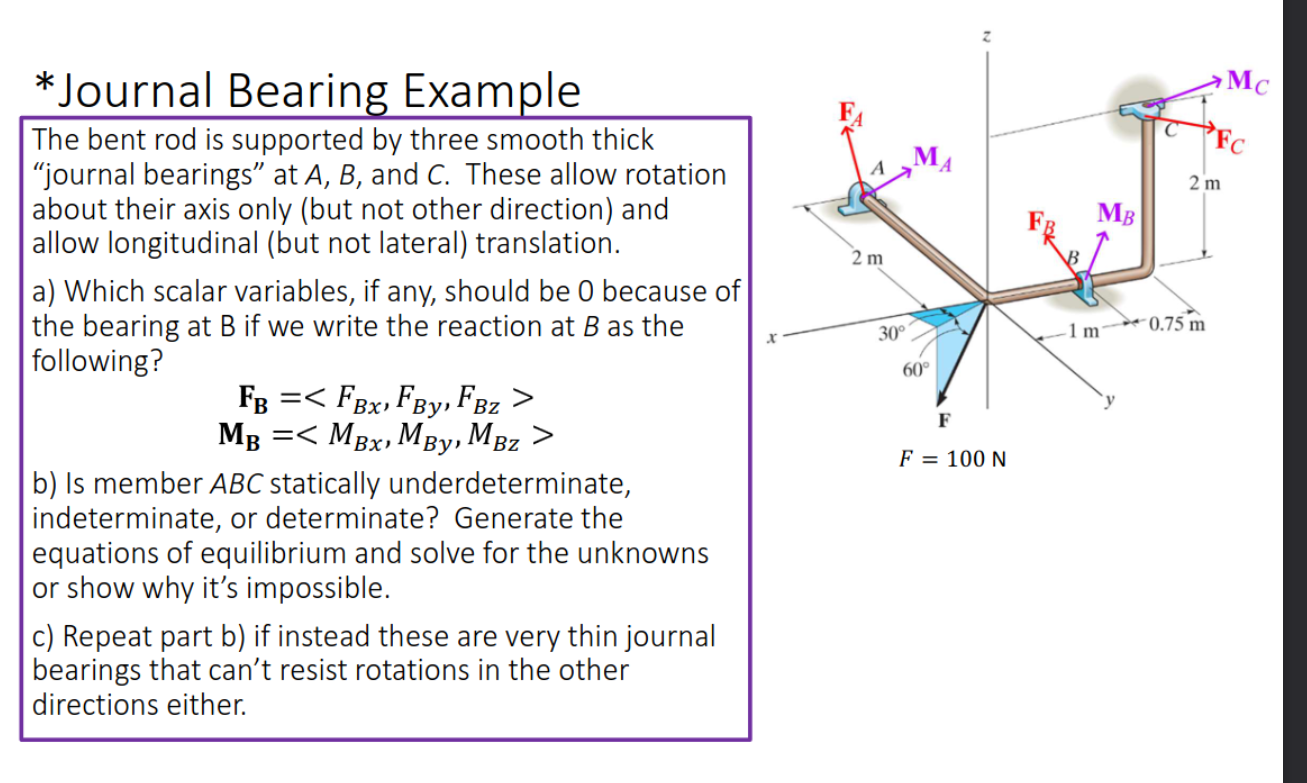
\includegraphics[width=15cm]{l6-lq1.png}

For part A, we can start by realizing that the reaction at B has no x component, the reaction at A has no y component, and the reaction at C has no z component.
This is true for both the forces and the moments.
This is because of the way the journal bearings are set up.

Now we can create an equation for net torque and an equation for the net force, both of which should be equal to 0.
However, in spite of this, we have 12 unknowns: the 2 moment components and the 2 force components at each of the 3 points.
This isn't possible since we can only create 6 equations from the net force and net torque equations.
Therefore, this system is statically indeterminate (more unknowns than equations).

Now if we had very thin journal bearings, we could assume that the moments at A, B, and C are 0.
Now we have 6 unknowns and 6 equations, which is solvable.
So let's do so in Maple:

\begin{lstlisting}[language=matlab, basicstyle=\small]
	restart: with(LinearAlgebra):
	FA:=<FAx,0,FAz>: rA:=<0,-2,0>:
	FB:=<0,FBy,FBz>: rB:=<-1,0,0>:
	FC:=<FCx,FCy,0>: rC:=<-1.75, 0, 2>:
	F:=100*<cos(Pi/3)*cos(Pi/6), cos(Pi/3)*sin(Pi/6), sin(Pi/3)>:
	Fnet:=FA+FB+FC+F:
	TauNet:= rA &x FA + rB &x FB + rC &x FC: # Moments are 0 so no need to add
	solve([Fnet[1]=0,Fnet[2]=0,Fnet[3]=0,TauNet[1]=0,TauNet[2]=0,TauNet[3]=0]);
\end{lstlisting}

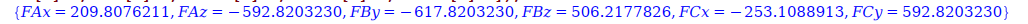
\includegraphics[width=15cm]{l6-lq1-o.png}

With this we've been given all of the forces.

\subsection{Quiz and Reflection}

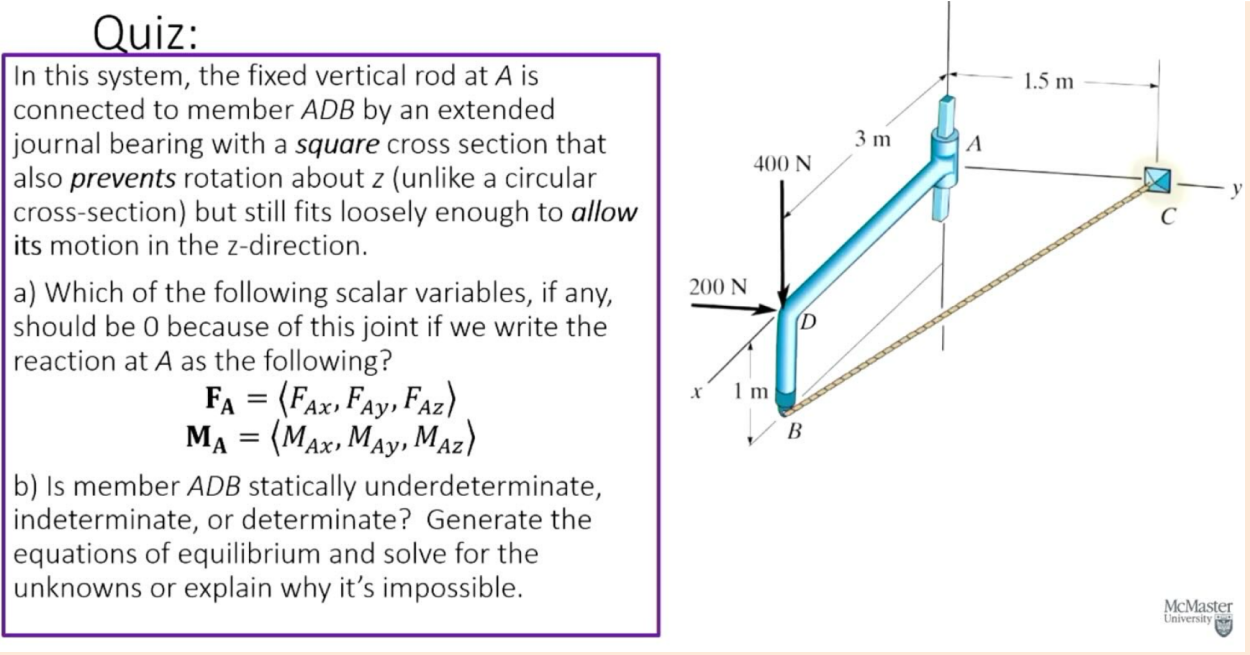
\includegraphics[width=15cm]{l6-quiz.png}

For part A, we know that point A only allows motion along the z axis.
That is why the reaction force at A only has x and y components--$F_{Az}$ is 0.

\begin{lstlisting}[language=matlab, basicstyle=\small]
	restart: with(LinearAlgebra):
	Fa:=<Fax,Fay,0>:Ma:=<Max,May,Max>:
	# Define other points with reference to A (origin)
	rB:=<3,0,-1>:rC:=<0,1.5,0>:rD:=<3,0,0>:
	# Rope length vector and unit vector
	rBC:=rC-rB:rBC_hat:=rBC/sqrt(rBC.rBC):
	Fbc:=T*rBC_hat: # Force of tension
	Fd:=<0,200,-400>: # Force actin at point D
	Fnet:=Fa+Fd+Fbc; # All forces acting on system (sum 0)
	TauNet:= rB &x Fbc + rD &x Fd + Ma; # Torque around origin
	solve([Fnet[1], Fnet[2], Fnet[3]]);
\end{lstlisting}

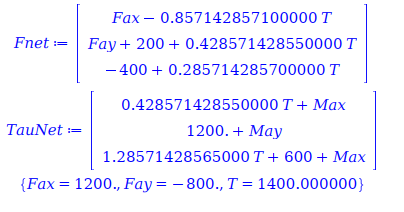
\includegraphics[width=10cm]{l6-quiz-o.png}

Therefore, we found some of the unknown values. 
With the TauNet equation, we can find the rest of the unknowns as well.

\medskip

Reflection: In this lecture we learned about how to solve statically indeterminate systems by assuming that the moments at certain points are 0.
This allows us to solve for the unknowns in the system.
We also learned about how to solve for the forces in a system when we have a system of equations that we can solve for the unknowns in.

\subsection{Problem Bank}

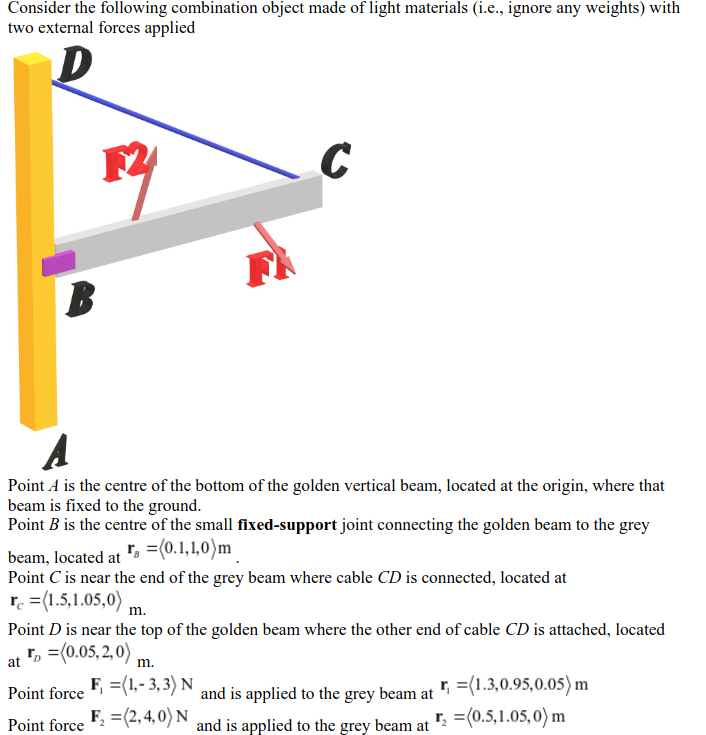
\includegraphics[width=15cm]{l6-pbq.png}

Part A: The system itself seems to be statically determinate.
This is because the only unknown seems to be the reaction force at point A.
When looking at the grey beam, however, the system changes to be statically indeterminate.
This is because there are more unknowns than the number of equations we can create for the beam.

Part B: Reaction force of A is opposite the net force from $F_1$ and $F_2$ and the reaction moment is opposite the net torque from $F_1$ and $F_2$.

Part C: We can introduce a new reaction force at B and see how $F_1$, $F_2$, and $F_B$ interact with each other to keep the system in equilibrium.

\begin{lstlisting}[language=matlab, basicstyle=\small]
	restart:with(LinearAlgebra):
	F1:=<1,-3,3>:r1:=<1.3,0.95,0.05>:
	F2:=<2,4,0>:r2:=<0.5,1.05,0>:
	FA:=-(F1+F2); # Reaction force
	MA:=-(r1 &x F1 + r2 &x F2); # Reaction moment

	# Part C
	rB:=<0.1,1,0>:
	rC:=<1.5,1.05,0>:
	rD:=<0.05,2,0>:
	FB:=<FBx,FBy,FBz>:
	MB:=<MBx,MBy,0>: # It's a pin hence the 0
	Fnet:=F1+F2+FB:
	# Torque about A
	tau_A:=r1 &x F1 + r2 &x F2 + (rB-rC) &x FB + MB:
	solve([Fnet[1], Fnet[2], Fnet[3], tau_A[1], tau_A[2], tau_A[3]]);
\end{lstlisting}

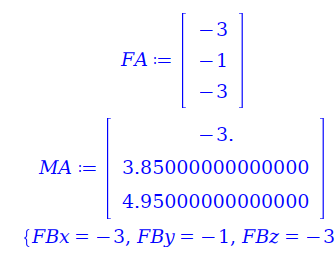
\includegraphics[width=10cm]{l6-pbq-o.png}

Part D: Given our answer, we know that the opposite of the net force must be the reaction force at A and B respectively.
We notice that the only forces (apart from the reaction forces) are $F_1$ and $F_2$. Therefore, it makes sense that the reaction force at A and B are equal to the net force of $F_1$ and $F_2$, and are therefore equal to each other.
This agrees with Newton's third law, which states that for every action there is an equal and opposite reaction.
In this case, the equal and opposite reaction is the reaction force at A and/or B depending on context

\section{Lecture 7}

\subsection{Problem Bank}

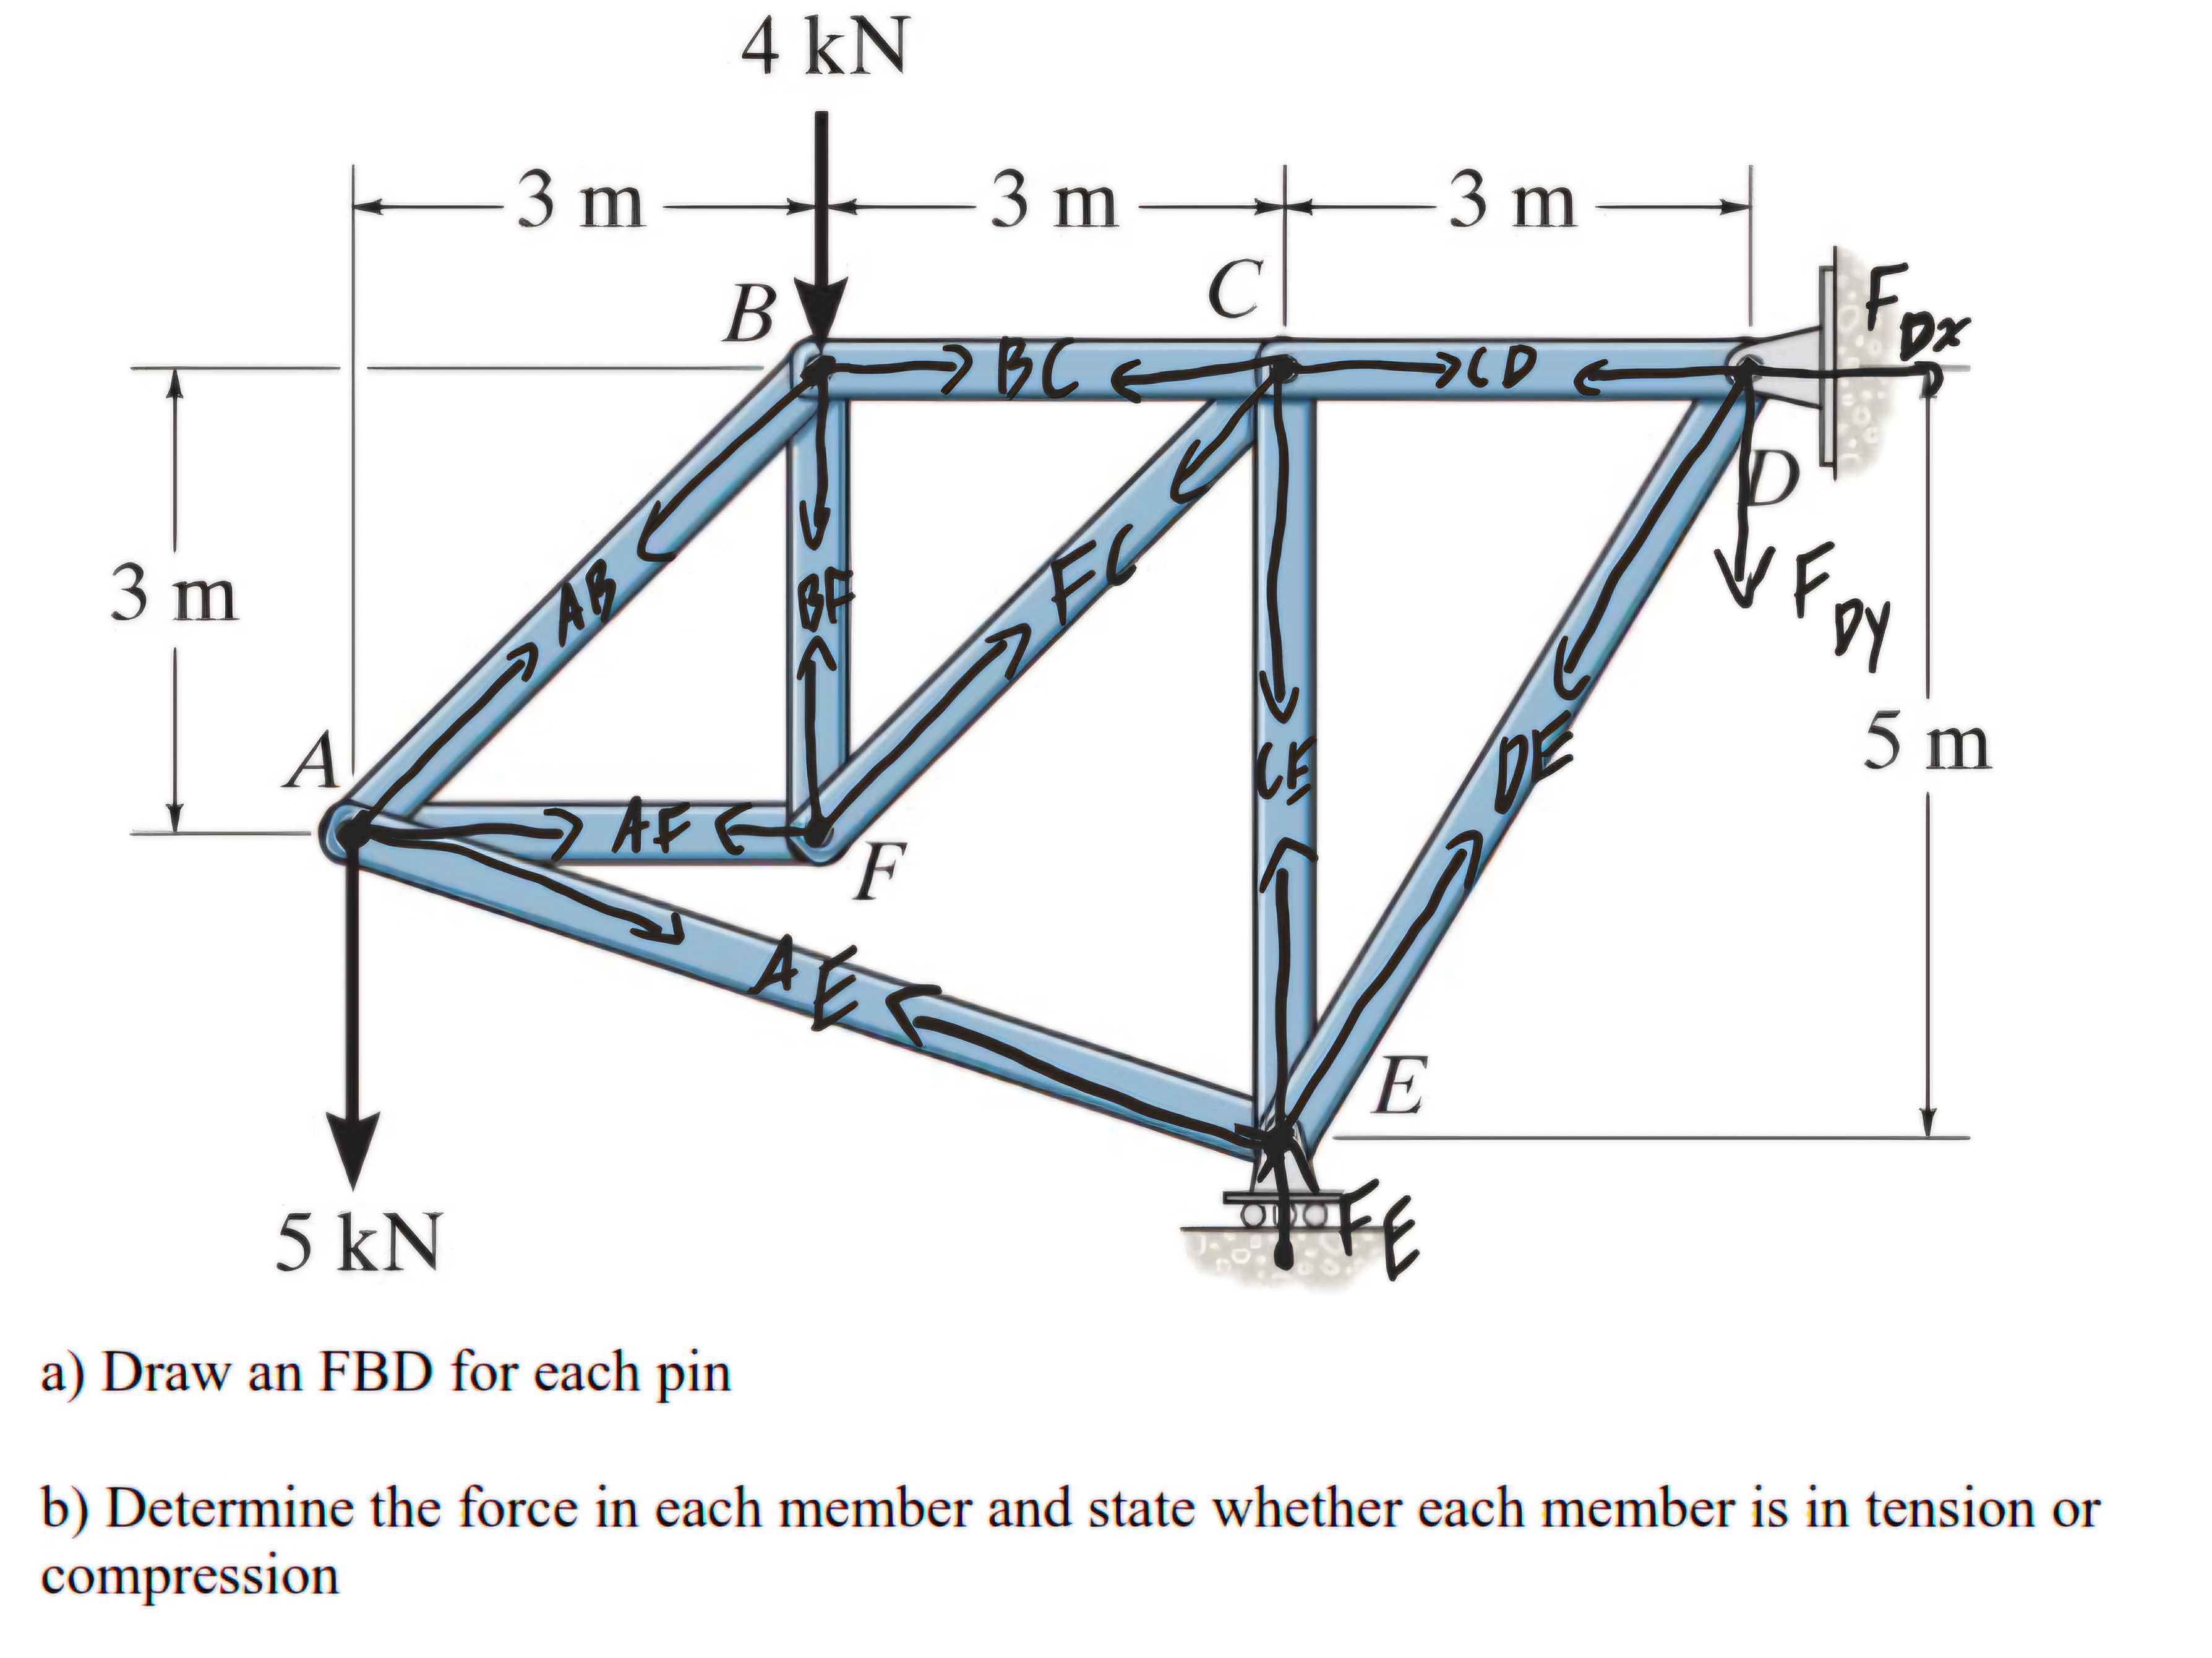
\includegraphics[width=15cm]{l7-pbq.png}

We can write Maple code with all the equations and solve for the individual forces in each member.
The compressive forces will be the negative values of the forces, while the tensile forces will be the positive values of the forces.
We will make the forces pointing right and forces pointing up positive in our Maple code.
We can use basic trig to find the DE, AF, FC, and AE forces' components when we subtract or add them to other forces at that point to reach equilibrium.
We have the following code:

\begin{lstlisting}[language=matlab]
	restart; 
	evalf(solve([
		3 * FC / sqrt(18) + BF = 0, 
		-4000 - 3 * AB / sqrt(18) - BF = 0, 
		-3 * AB / sqrt(18) + BC = 0, 
		-6 * AE / sqrt(40) + 3 * DE / sqrt(34) = 0, 
		-5 * DE / sqrt(34) - Fdy = 0, 
		Fdx - CD - 3 * DE / sqrt(34) = 0, 
		-3 * FC / sqrt(18) + CD - BC = 0, 
		-2 * AE / sqrt(40) + 3 * AB / sqrt(18) - 5000 = 0, 
		3 * FC / sqrt(18) - AF = 0, 
		5 * DE / sqrt(24) + 2 * AE / sqrt(40) + CE + Fey = 0, 
		-6 * AE / sqrt(40) + 3 * DE / sqrt(34) = 0, 
		-3 * FC / sqrt(18) - CE = 0, 
		AF + 3 * AB / sqrt(18) + 6 * AE / sqrt(40) = 0
	]));
\end{lstlisting}

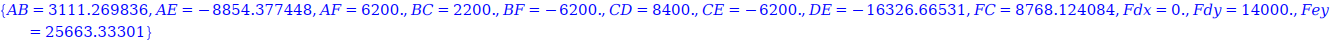
\includegraphics[width=15cm]{l7-pbq-o.png}

Now we have the force on each component and we know that the compressive forces are AE, BF, CE, DE since those forces are negative.

\section{Lecture 8}

\subsection{Problem Bank}

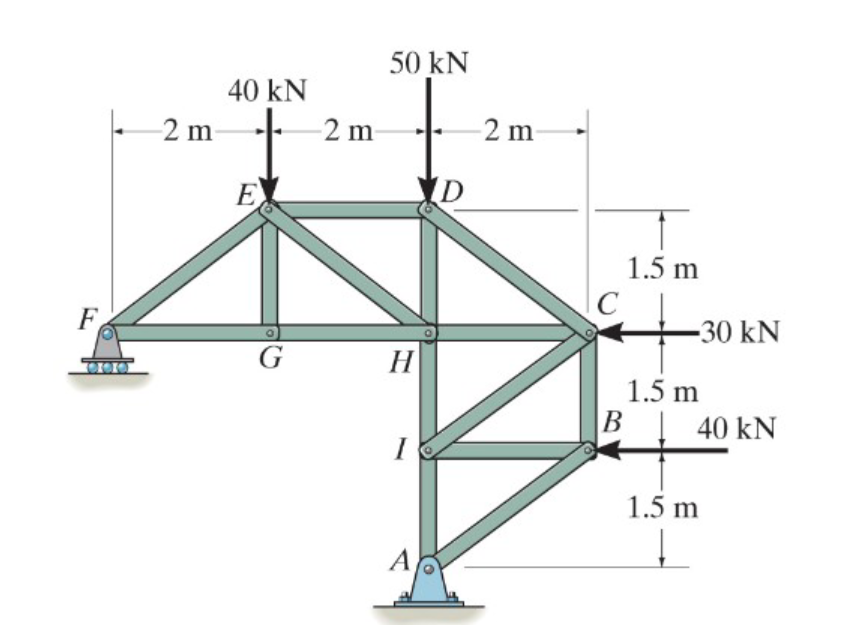
\includegraphics[width=15cm]{l8-pbq.png}

We can start off by acknowledging that the net force in the x and y directions must be 0 and the net torque around point A must also be 0.
We can start by finding the reaction forces from points F and A which must keep the system in equilibrium.
We can then find the forces in the members by using the equations of equilibrium.
Maple code:

\begin{lstlisting}[language=matlab]

	restart:
	Fnet_y:=Fy-50000-40000+Ay:
	Fnet_x:=Ax-30000-40000:
	tau_netA:=Fy*4 - 40000*1.5 - 30000*3 - 40000 * 2:
	vals:=solve([Fnet_y,Fnet_x,tau_netA]); # vals[3] = Fy

	FNET_X:= ED + GH + EH * 2 / sqrt(2^2 + 1.5^2): # X forces at E
	FNET_Y:= 57500 - 40000 - EH * 1.5/sqrt(2^2+1.5^2): # Y forces E
	tau_e := 2 * 57500 - 1.5 * GH: # Torque around E should be 0
	solve([FNET_Y, FNET_X, tau_e]): evalf(%);


\end{lstlisting}

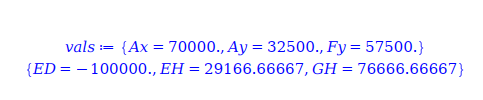
\includegraphics[width=15cm]{l8-pbq-o.png}

What's happening is that we initially create 3 equations for the net forces in the x and y directions and the net torque around point A.
From that equation, we're able to solve for the net force in the y direction acting on point F.
With that, we can solve for the net x force acting on that area, the net y force acting on that area, and the torque acting on point E in that specific area.
We have 3 unknowns and 3 equations, so we can solve for the forces in the members.

From the output, we can see that EH and GH are tensile forces while ED is a compressive force since it is negative.

\end{document}
